\section{Hypothèses et modèle}

\begin{figure}[h]
    \caption{Modèle synthétique}
    \label{fig:modelsynth}
    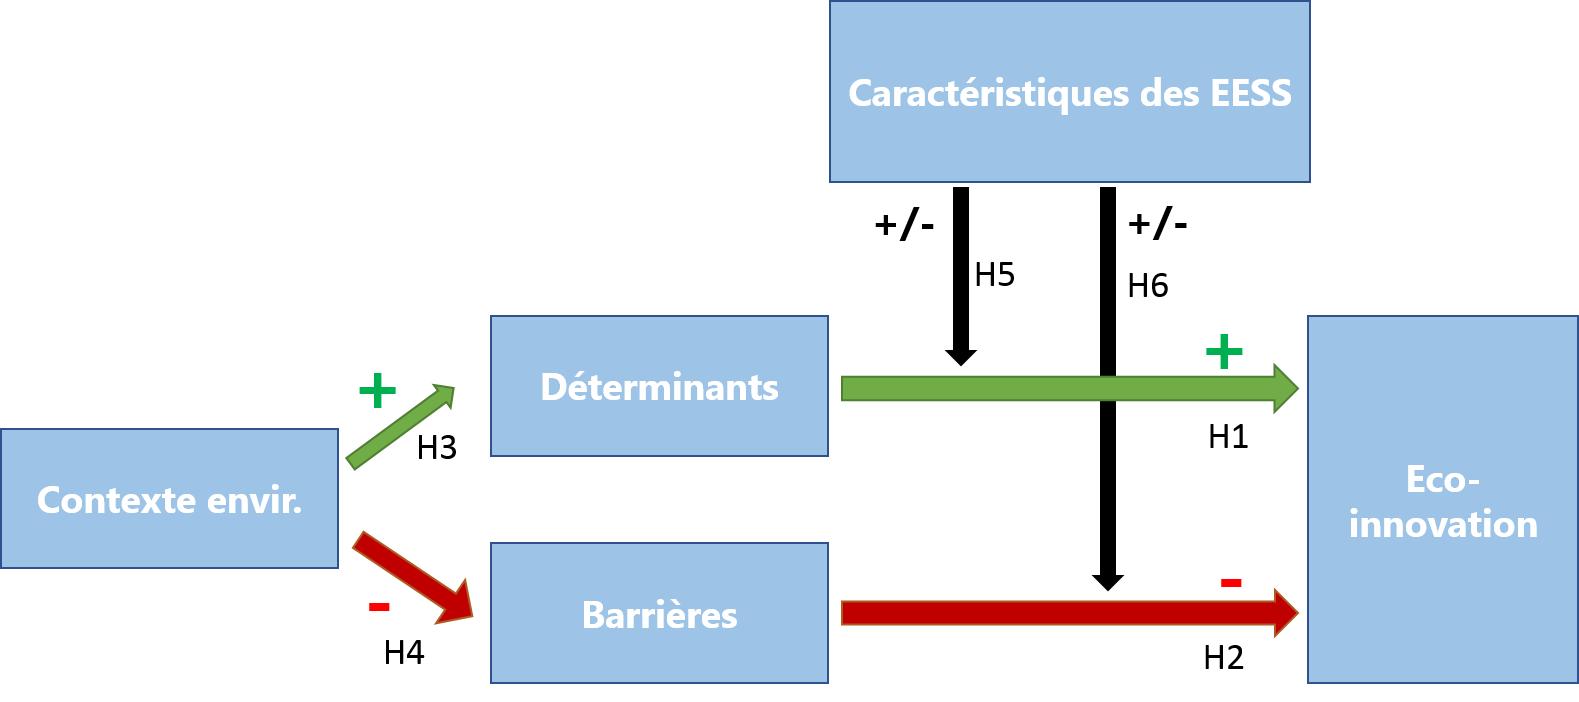
\includegraphics[width=\linewidth]{fig/Modele/model1.png}
\end{figure}

\begin{figure}[h]
    \caption{Modèle : déterminants de l'éco-innovation}
    \label{fig:modeldet}
    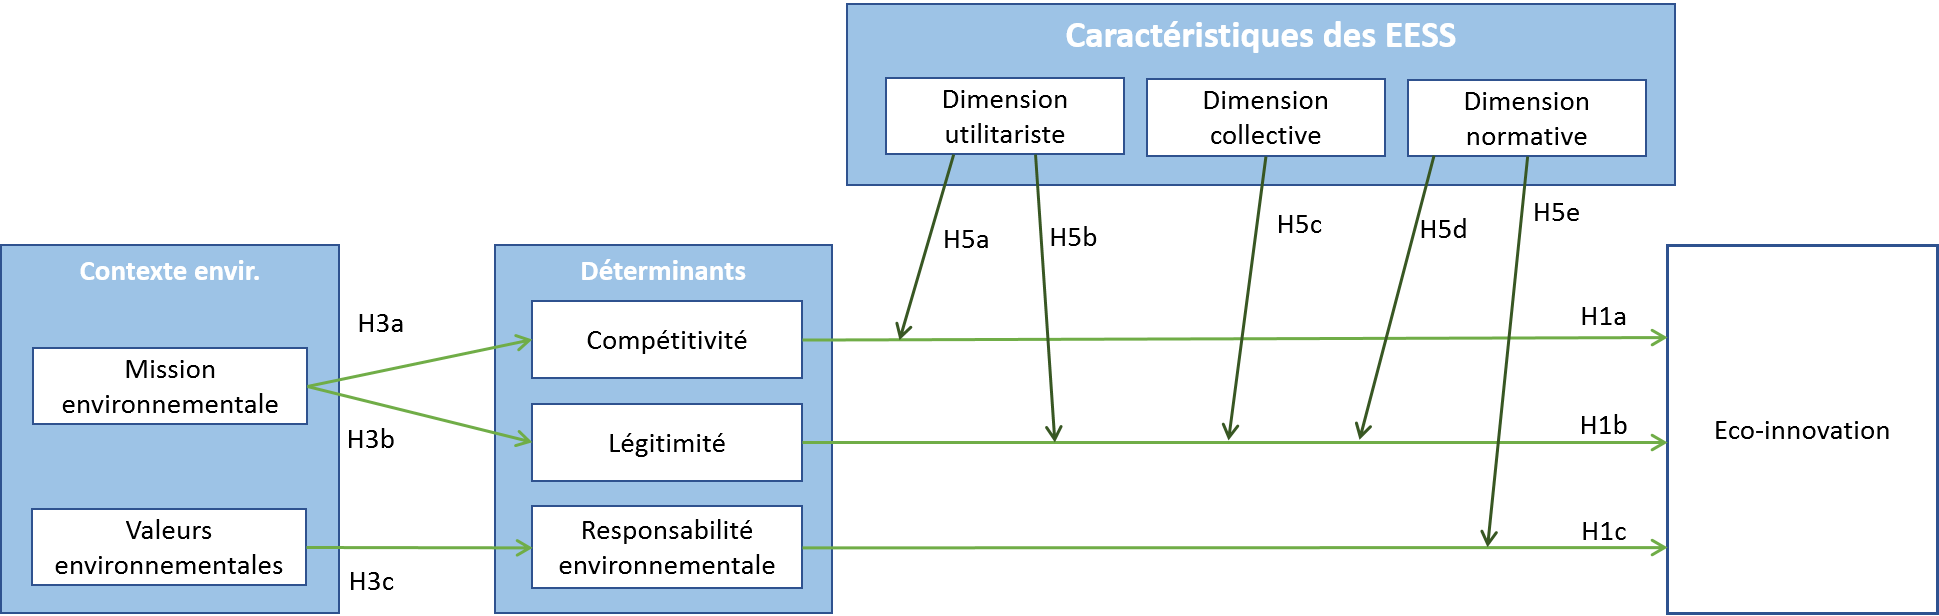
\includegraphics[width=\linewidth]{fig/Modele/model2.png}
\end{figure}

\begin{figure}[h]
    \caption{Modèle : Barrières à l'éco-innovation}
    \label{fig:modelbar}
    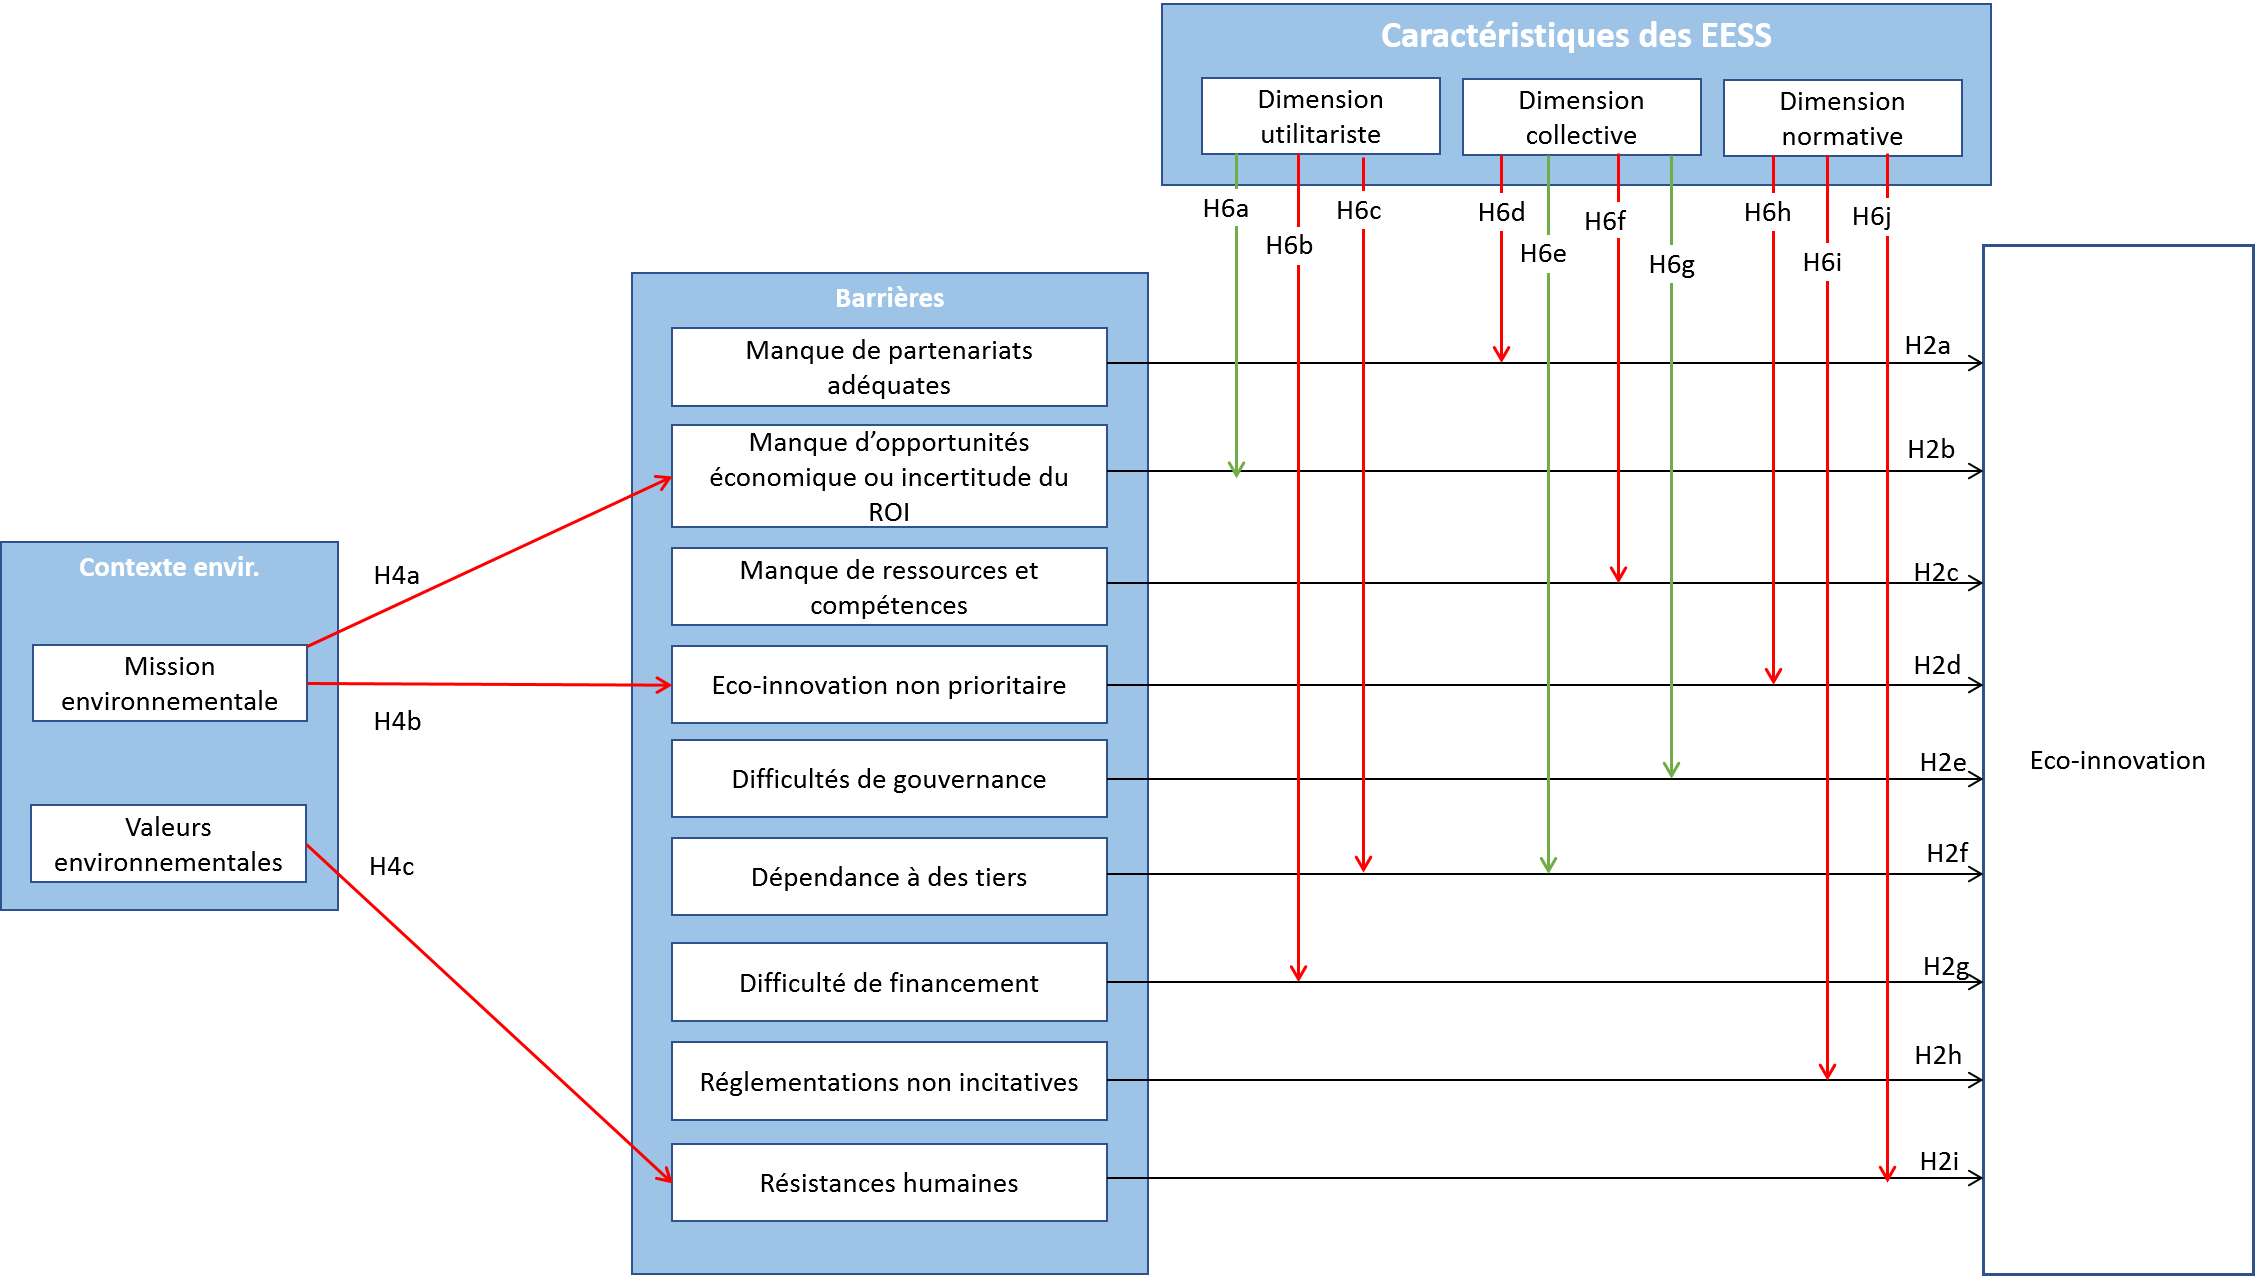
\includegraphics[width=\linewidth]{fig/Modele/model3.png}
\end{figure}

Dans cette section, nous formulons des hypothèses de recherche qui seront testées dans la phase confirmatoire de l’étude. Celles-ci s’appuient tout d’abord sur les éléments de la littérature. Toutefois, les recherches faisant un lien direct entre les caractéristiques des EESS et l’éco-innovations sont peu nombreuses. C’est pourquoi nous nous appuyons également sur les deux recherches exploratoires menées en amont. L’exploration du contenu de Twitter nous renseigne sur les différentes approches des questions environnementales selon les caractéristiques des EESS. L’étude de cas permet d’approfondir ces résultats en identifiant clairement ces caractéristiques selon les dimensions normative, utilitariste et collective, et en y associant les motivations à l’éco-innovation correspondantes. 

Le Tableau \ref{} synthétise les hypothèses qui sont développées dans les paragraphes suivants. Nous précisions pour chacune les principaux supports issus de la littérature et ceux issus des études exploratoires.

\todo[inline]{Tableau et développement des hypothèses}

\section{Questionnaire}

Nous avons étudié la littérature relative à l’éco-innovation et à l’ESS, puis nous avons mené deux études exploratoires visant à approfondir les liens entre ces deux concepts. Ceci nous a permis de définir XX hypothèses, que nous souhaitons tester. Pour cela nous avons recours à une étude quantitative confirmatoire. Dans cette partie, nous décrivons la constitution de l’instrument de mesure, à savoir le questionnaire de recherche. Cette phase s’inscrit dans le paradigme de Churchill : à partir des études exploratoires, nous adaptons les échelles de mesure existantes, et nous générons un jeu d’items pour les concepts pour lesquels aucune échelle n’est disponible dans la littérature. Conformément à ce qui est préconisé par Churchill, une première collecte permettra de tester et de purifier le questionnaire, avant de le diffuser à un échantillon plus large de répondants. 

\subsection{Echelles relatives aux dimensions de l’ESS}

Nous n’avons pas identifié d’échelles permettant de caractériser l’ESS selon les trois dimensions de notre modèle. Les items sont donc générés à partir de la littérature enrichie par les études préliminaires (Tableau \ref{table:itemdimensions}). Pour la dimension utilitariste, nous avons identifié quatre éléments distinctifs : les sources de revenus, les ressources humaines, le caractère professionnel et formalisé, et l’utilisation des bénéfices. La dimension collective est caractérisée par l’importance donnée aux partenariats, la participation des salariés aux décisions, et l’ouverture de la gouvernance à des parties prenantes externes. La dimension normative repose sur l’attachement à des valeurs sociales et solidaires, la poursuite d’une mission d’intérêt général, et une volonté de transformation de la société et de l’économie. 

Pour ces items, on utilisera une échelle de Likert en 7 points (Pas du tout d’accord, Pas d’accord, Plutôt pas d’accord, Ni d’accord ni pas d’accord, Plutôt d’accord, d’accord, Tout à fait d’accord). 

\begin{landscape}
\begin{longtable}{
    |>{\setlength{\baselineskip}{0.6\baselineskip}}K{0.25\linewidth}
    |>{\setlength{\baselineskip}{0.6\baselineskip}}K{0.15\linewidth}
    |>{\setlength{\baselineskip}{0.6\baselineskip}}K{0.50\linewidth} |
    }
    \caption{Synthèse des items : dimensions de l'ESS}
    \label{table:itemdimensions} \\ 
    \hline
    
        \textbf{Item} & \textbf{Code item }& \textbf{Commentaire} \\ \hline
        \endfirsthead 
        \hline
         \textbf{Item} & \textbf{Code item }& \textbf{Commentaire} \\ \hline
         \endhead
         
         \multicolumn{3}{|l|}{\textbf{Dimension utilitariste}} \\ \hline
         
         Nos revenus proviennent en majorité d’une activité commerciale (vente de produits et/ou services) & ut\_rev\_act &    La question des modalités de financement est une caractéristique majeure de l’ESS. Le possible recours à des subventions ou à des dons différencient nettement les EESS des entreprises du secteur capitaliste \parencite{dart2004being}. \newline
        L’étude de cas montre que les EESS s’inscrivant dans une démarche utilitariste, visant à s’appuyer sur la performance et à garantir une indépendance économique cherchent à maximiser les sources de revenus issus de leur activité commerciale.  \\ \hline
        
        Nos revenus proviennent en majorité d’une activité sous agrément (délégation de service public…) & ut\_dsp & Item ajouté à la suite de l’entretien d’expert : mode de financement particulier qui n’est pas une subvention mais pas un revenu de marché non plus et qui est fréquent dans l’ESS, notamment dans le secteur de la Santé. \\ \hline
        
        Notre activité dépend fortement de personnes bénévoles et/ou en contrat aidé et/ou en service civique   & ut\_ben & De la même façon, le recours à des bénévoles ou à des contrats aidés ne correspond pas à des pratiques de marché mais constitue une spécificité de certaines EESS \parencite{salamon2016beyond}. Pour \textcite{demoustier2003lentreprise}, le bénévolat est caractéristique de modes de production distincts de la production marchande lucrative. \newline
        Au cours de l’étude de cas, un répondant a indiqué qu’il n’avait pas recourt au bénévolat car il dirigeait « des associations entrepreneuriales », mettant ainsi le doigt sur une divergence dans les approches de l’économie sociale. 
        Item reformulé à la suite de l’entretien d’expert\\ \hline
        
        Nos prix d'achat et de vente sont basés exclusivement sur l'offre et la demande (prix de marché) & ut\_prix &    \textcite{demoustier2003lentreprise} soulignent le recourt possible à la tarification particulière dans l’ESS, en fonction des revenus par exemple.  \newline
        Dans l’étude de cas, plusieurs organisations établissent les prix autrement que par le marché. Enercoop revendique un tarif plus élevé mais plus « juste » pour le service écologique rendu. Le commerce équitable est un exemple de secteur ou les prix d’achats sont également supérieurs à ceux du marché.\\ \hline
        
        Notre activité est menée de manière très professionnelle et formalisée  & ut\_form & Les EESS utilitaristes soulignent leur dimension professionnelle. Différents points de vue s’opposent au sein de l’ESS. Pour les tenant du managérialisme, l’application des méthodes de gestion du secteur privé classique est considérée comme plus efficaces. D’autres en revanche dénoncent ces pratiques et s’inquiète du risque de perdre de vue la mission initiale de l’entreprise \parencite{eikenberry2009refusing}. Dans l’étude de cas, le Président d’Arborescence a insisté sur le fait que le fonctionnement d’une EESS est similaire à celui d’une entreprise classique, et qu’une organisation hiérarchique, avec un « chef » est indispensable. Au contraire, un co-Président de l’association Bzzz se présente comme \cit{un patron différent}. \\ \hline
        
        Notre organisation se fixe des objectifs de croissance et de développement & ut\_croiss & \textcite{dart2004being,maier2016nonprofit} identifient la fixation d’objectifs en des termes commerciaux comme un des éléments caractéristiques d’une tendance à la transformation de l’ESS vers un fonctionnement de marché. Dans l’étude de cas, les EESS fortement utilitaristes affichent des ambitions de croissance et de développement, notamment par croissance externe. Au contraire, les entreprises peu utilitaristes fixent plutôt des objectifs relatifs à leur mission sociale, les aspects économiques étant une contrainte à respecter plutôt qu’une finalité. \\ \hline
        
        Les investisseurs, sociétaires ou coopérateurs attendent un retour sur investissement & ut\_benef &  La non lucrativité est une caractéristique majeure de l’ESS dont la finalité est la mission sociale ou environnementale et non la création de valeur financière. Toutefois, la distribution des profits est possible dans certaines structures dès lors qu’elle bénéficie à des acteurs engagés dans l’organisation (coopérateurs, sociétaires). La vision moderne de l’entrepreneuriat social admet aussi la distribution de profits à des investisseurs, de manière limitée, afin d’ouvrir à l’ESS de nouveaux modes de financement \parencite{salamon2016beyond}. \\ \hline
        
        \multicolumn{3}{|l|}{} \\ \hline
        \multicolumn{3}{|l|}{\textbf{Dimension collective}} \\ \hline
        
        L'organisation mène des projets en collaboration avec de nombreux partenaires	&	col\_part	&	L’étude de cas suggère que les organisations s’inscrivant dans une logique collective multiplient les partenariats. Toutefois, cette notion peut renvoyer aux fournisseurs, clients, financeurs, membres… Cet item valorise l’idée de collaboration, qui met en avant la volonté de « faire ensemble », qui va plus loin qu’une relation de marché de type client-fournisseur ou financé-financeur. 	\\ \hline
        Les salariés prennent part aux décisions stratégiques de l'organisation	&	col\_sal	&	"Les salariés occupent une place particulière au sein de l’entreprise. Toutefois, les statuts de l’ESS n’imposent pas que les salariés soient impliqués dans les décisions de l’entreprise.  \newline
        Dans l’étude de cas, la volonté exprimée par certaines organisations de donner aux salariés une place dans la gouvernance traduit une véritable volonté de mettre en place un projet collectif."	\\ \hline
        Les décisions sont prises de manière complètement démocratique	&	col\_dem	&	Le principe de démocratie est au cœur des valeurs de l’ESS et caractérise sa volonté collective. L’adjectif « complètement » vise à augmenter l’aspect discriminant de cet item : il vise à mesurer si l’organisation va au-delà de ce qui est imposé par son statut. 	\\ \hline
        Les organes de gouvernance intègrent de nombreuses parties prenantes (clients, fournisseurs, société civiles, collectivités, salariés...)	&	col\_pp	&	Les statuts de l’ESS imposent une logique démocratique (« une personne = une voix ») mais ne contraignent pas les organisations à faire apparaitre une diversité de parties prenantes. Certains statuts comme celui de SCIC prévoient toutefois une ouverture très large de la gouvernance. Là encore, l’ouverture à des acteurs externes traduit la volonté de ne pas agir de manière isolée, mais de répondre le plus largement possible à des attentes multiples. 	\\ \hline
        Les décisions résultent d'un consensus entre toutes les parties prenantes 	&	col\_dec	&	"Cet item vise à renforcer la notion de démocratie, celle-ci étant légalement commune à toutes les EESS. \newline
        Un des cas étudiés applique la règle du consensus. Ceci montre que l’entreprise souhaite aller plus loin et mettre en œuvre des solutions bénéfiques à toutes les parties prenantes. "	\\ \hline
        Notre mission est de répondre conjointement aux attentes de nos clients, de nos salariés, de nos fournisseurs ainsi que de nos partenaires	&	col\_att	&		\\ \hline
        
        \multicolumn{3}{|l|}{} \\ \hline
        \multicolumn{3}{|l|}{\textbf{Dimension normative}} \\ \hline
        
        Notre organisation donne la priorité à l'intérêt général	&	norm\_intgen	&	Bien que l’ESS soit fréquemment définie comme un champ visant à contribuer à l’intérêt général, certains préfèrent parler \cit{d’intérêt collectif}. En effet certaines formes organisationnelles ont vocation à mutualiser les moyens dans l’intérêt premier de leurs membres. Cet item mesure donc la volonté d’avoir un impact sociétal. 	\\ \hline
        Notre organisation propose une nouvelle vision de la société	&	norm\_soc	&		\\ \hline
        Notre organisation défend une économie alternative	&	norm\_alter	&	Ces deux items renvoient à la dimension transformatrice de l’économie proposée par l’ESS \parencite{laville2016economie}. Les EESS s’inscrivant dans cette démarche ne cherchent pas simplement à conduire leur activité, mais à proposer une autre vision de la société. 	\\ \hline
        Notre organisation a une dimension politique et militante	&	norm\_milit	&	Plusieurs des cas étudiés mettent en avant une approche alternative de l’économie. 	\\ \hline
        Nous revendiquons notre appartenance à l’économie sociale et solidaire	&	norm\_ess	&	Toutes les entreprises ne revendiquent pas leur appartenance à l’ESS. 	\\ \hline
        Notre organisation revendique son adhésion à des valeurs de solidarité, de démocratie et d’humanisme	&	norm\_valeurs	&	L’étude de cas révèle que certaines n’ont pas conscience d’en faire partie, quand bien même elles rentrent de fait dans son périmètre. Le fait de revendiquer l’appartenance à l’ESS permet de mettre en avant la spécificité normative de l’entreprise. Le second item mesure en particulier l’attachement aux valeurs qui résulte de cette appartenance à l’ESS. Dans les documents étudiés, l’appartenance au champ de l’économie social renvoie en effet en premier lieu à ses valeurs. 	\\ \hline
        Appartenir à l’économie sociale et solidaire est un fondement indispensable de notre entreprise	&	norm\_fondement	&	Le choix d’un statut d’ESS peut être pragmatique (statut perçu comme le plus favorable ou le plus adapté à l’activité) comme il peut résulter d’une volonté de marquer une réelle différence de philosophie d’entreprise. Cet item vise à valoriser ce second cas. 	\\ \hline

\end{longtable}
\end{landscape}

\subsection{Echelles relatives aux pratiques d’éco-innovation }

Cette partie du questionnaire vise à déterminer si l’entreprise est généralement éco-innovante. \textcite{arundel2009measuring} soulignent la difficulté de mesurer l’éco-innovation et proposent différentes approches. Une solution communément adoptée est de s’appuyer sur des études menées à grande échelle par des organismes internationaux. Nous nous appuyons ici sur une partie du questionnaire \cit{Flash Eurobarometer 315 - Attitudes of European Entrepreneurs Towards Eco-innovation} de la Commission Européenne \footnote{European Commission, 2011. “Flash Eurobarometer 315, Attitudes of European Entrepreneurs Towards Eco-innovation”, Survey Conducted by the Gallup Organization, Budapest (Producer), January 2011. GESIS, Cologne. \url{http://dx.doi.org/10.4232/1.10747} (ZA5470, dataset version 1.0.0, Report: \url{http://ec.europa.eu/public_opinion/flash/fl_315_en.pdf})}, qui est repris notamment par \textcite{triguero2013drivers}. Toutefois, au regard des résultats des études exploratoires, il nous a semblé nécessaire de compléter cette partie avec de nouveaux items afin d’élargir à différents types d’éco-innovations. Les questions adaptées et complétées sont présentées dans le Tableau \ref{table:pratiquesEI}. Nous avons souhaité également mesurer la portée de l’éco-innovation (intensité de l’innovation et volonté de diffusion), pour laquelle nous n’avons pas identifié d’échelles pertinente et interroger les répondants sur les modes de financements utilisés. De nouveaux items ont donc été générés à partir des études préliminaires et de la littérature (tableaux \ref{table:porteeEI} et  \ref{table:financementEI}). 

{\small
\begin{landscape}
\begin{longtable}{
    |>{\setlength{\baselineskip}{0.6\baselineskip}}K{0.28\linewidth}
    |>{\setlength{\baselineskip}{0.6\baselineskip}}K{0.28\linewidth}
    |>{\setlength{\baselineskip}{0.6\baselineskip}}K{0.28\linewidth}
    |>{\setlength{\baselineskip}{0.6\baselineskip}}K{0.10\linewidth} |
    }
    \caption{Synthèse des items : pratiques d'éco-innovation}
    \label{table:pratiquesEI}  \\ 
    
    \hline
        \textbf{Item original} & \textbf{Item adapté}& \textbf{Commentaire} & \textbf{Code item} \\ \hline
        \endfirsthead 

        \hline
         \textbf{Item original} & \textbf{Item adapté}& \textbf{Commentaire} & \textbf{Code item} \\ \hline
         \endhead
         
        D5. Au cours des 24 derniers mois avez‐vous introduit les éco‐innovations suivantes :& 	Au cours des 24 derniers mois, avez-vous mené les actions environnementales suivantes ?	& Échelle modifiée : \citit{Jamais -, une seule fois - plusieurs fois - de nombreuses fois}&\\ \hdashline
        
            \citit{a. un produit ou un service éco‐innovant nouveau ou considérablement amélioré sur le marché.} &	\citit{Évolutions de vos produits ou services}
            & \multirow[c]{3}{\hsize}[-1.2cm]{\begin{spacing}{1}On considère l'éco-innovation au niveau de l'entreprise, et non au niveau du marché en général\end{spacing}} & typ\_prod \\ \cdashline{1-2} \cline{4-4}
            
            \citit{b. une méthode ou un processus de production éco‐innovant nouveau ou considérablement amélioré} &	\citit{Évolutions de vos méthodes ou processus de production}&& typ\_process \\ \cdashline{1-2} \cline{4-4}
            
            \citit{c. une innovation organisationnelle éco‐innovante nouvelle ou considérablement améliorée} & 	\citit{Changements organisationnels (par exemple : certification environnementale, réorganisation des services, changement de fournisseurs...)} &&typ\_orga \\ \hdashline
            
            &  \citit{Actions portant sur les pratiques ou les comportements individuels de vos salariés, bénéficiaires ou clients} & \multirow{3}{\hsize}{\begin{spacing}{1}Items ajoutés pour inclure les éco-innovations sociale et institutionnelle dont plusieurs exemples ont été observés dans l’étude de cas\end{spacing}} & typ\_social  \\ \cdashline{1-2} \cline{4-4}
            
            & Actions impliquant des changements pour l'ensemble d'une filière, ou aboutissant à une modification de la réglementation en vigueur&&typ\_instit \\ \hline
            
        Q6. Au cours des 5 dernières années, quelle part de l’investissement d’innovation dans votre entreprise était en rapport avec l’éco‐innovation, c’est‐à‐dire mise en oeuvre de solutions nouvelles ou considérablement améliorées entraînant une utilisation plus efficace des matériaux, de l’énergie et de l’eau ? &	Au cours des 5 dernières années, quelle part de l'investissement a concerné l'action environnementale ? &	Nécessité d'une vision plus générale de l'éco-innovation. Celle-ci est définie en préambule de la page du questionnaire correspondante. \newline Échelle initiale maintenue : \citit{Aucune – moins de 10\% - entre 10\% et 29\% - Entre 30\% et 49\% - Plus de 50\% - Pas d’activité innovante} &	env\_invest \\ \hline
         
\end{longtable}
\end{landscape}
}


{\small
\begin{landscape}
\begin{longtable}{
    |>{\setlength{\baselineskip}{0.6\baselineskip}}K{0.25\linewidth}
    |>{\setlength{\baselineskip}{0.6\baselineskip}}K{0.15\linewidth}
    |>{\setlength{\baselineskip}{0.6\baselineskip}}K{0.50\linewidth} |
    }
    \caption{Synthèse des items : portée de l'éco-innovation}
    \label{table:porteeEI} 
    
    \small \\ \hline
    \textbf{Item} & \textbf{Code item }& \textbf{Commentaire} \\ \hline
    \endfirsthead
    \hline
    \textbf{Item} & \textbf{Code item }& \textbf{Commentaire} \\ \hline
    \endhead

    Notre mission est directement liée à l'environnement &	envir\_mission	& Item ajouté à la suite de l’étude de cas : permet de distinguer les EESS qui ont une mission environnementale \\ \hline
    L’écologie fait partie de nos valeurs	& envir\_valeurs	& Item \\ \hline
    L'action environnementale est essentielle pour nous	& int\_importance &	Item général visant à déterminer si la stratégie de l’entreprise repose sur l’éco-innovation \\ \hline
    
    Nous consacrons une part importante de nos efforts à l'action environnementale	& int\_efforts	& \\ \hline
    Nous faisons régulièrement évoluer nos pratiques pour mieux prendre en compte l'environnement	& int\_pratiques	& \\ \hline
    Nous sommes très innovants en matière d'action environnementale	& int\_innov & \\ \hline
    
    
    En général, nous sommes pionniers en matière d'action environnementale	
    & int\_pionnier
    & \multirow[t]{3}{\hsize}[18pt]{\singlespacing
    La littérature distingue les entreprises ayant une stratégie proactive ou adaptative d’éco-innovation. L’innovation peut d’ailleurs être perçue à deux échelles : celle de l’organisation ou celle de la société. L’adaptation d’une innovation au niveau de l’organisation (mais qui peut déjà exister dans d’autres entreprises) est plus courante que l’adoption d’une pratique ou technologie n’existant nulle part ailleurs. \newline
    Parmi les cas étudiés, certains ont adopté des innovations déjà mises en place ailleurs. Le projet écolo-crèche d’Enfants et Loisirs représente un changement très important pour l’association, mais existe déjà ailleurs (il est porté dans de nombreuses crèches par l’association Ecolo-Crèche). En revanche, le directeur de la Tour du Valat indique \citit{ce qu’on a fait c’est assez innovant, il y a peu de gens qui l’ont mis en place}. } \\[15ex] \cline{1-2}
    
    En matière d'action environnementale, nous nous appuyons généralement sur ce qui a déjà été fait ailleurs &	 int\_suiveur	& \\[15ex] \hline
    Notre action environnementale prend souvent la forme de projets d'envergure importante pour notre organisation &	int\_chgt	& La littérature distingue les innovations incrémentales des innovations radicales, ces dernières étant plus rares. Sans que la distinction soit aussi nette, l’étude de cas a montré des exemples d’éco-innovation dont la portée est variée, allant de petites adaptations du quotidien (installation d’une poubelle pour le recyclages) à des innovations majeures (construction de nouveaux bâtiments éco-énergétiques ou innovations aboutissants à des évolutions légales). \\ \hline

\end{longtable}


\begin{longtable}{
    |>{\setlength{\baselineskip}{0.6\baselineskip}}K{0.25\linewidth}
    |>{\setlength{\baselineskip}{0.6\baselineskip}}K{0.15\linewidth}
    |>{\setlength{\baselineskip}{0.6\baselineskip}}K{0.50\linewidth} |
    }
    \caption{Synthèse des items : portée de l'éco-innovation}
    \label{table:financementEI} 
    \small \\  
    \hline

    \textbf{Item} & \textbf{Code item }& \textbf{Commentaire} \\ \hline
    \endfirsthead 
    \textbf{Item} & \textbf{Code item }& \textbf{Commentaire} \\ \hline
         \endhead
         
        Réponse à un appel à projets public ou privé 
        & 	fin\_ap	
        & \multirow{3}{\hsize}{\singlespacing L’étude de cas suggère que les difficultés financières rencontrées par les EESS peuvent être compensées par l’accès à des financements dédiés comme le crowdfunding ou la participation à des appels à projets réservés à l’ESS} \\ \cline{1-2}
        Crowd-funding solidaire (financement participatif sous forme de dons)	& fin\_crowd& \\ \cline{1-2}
        Soutien financier d'une organisation de l'ESS ou d'un mécène& 	fin\_mecenat& \\ \hline
         
\end{longtable}

\end{landscape}
}


\subsection{Déterminants de l’éco-innovation}

Les trois catégories de déterminants de l’éco-innovations identifiées par \textcite{bansal2000why} sont la légitimité, la compétitivité et la responsabilité. Il n’existe pas à notre connaissance d’échelle de mesure de ces déterminants. Cependant, \textcite{bronn2009corporate}, s’intéressant aux initiatives sociales des entreprises, aboutissent à trois facteurs similaires : la profitabilité, la légitimité et le caractère durable (\textit{sustainability}). Etant donné la proximité des thématiques et la forte similarité entre les définitions des facteurs dans ces deux études, les échelles proposées par Brønn et Vidaver-Cohen peuvent être utilisées pour mesurer les déterminants de l’éco-innovation. L’action environnementale fait en effet partie de la responsabilité sociale des entreprises, et peut être considérée ici comme un sous ensemble de l’initiative sociale. Le Tableau \ref{table:determinantsEI} reprends les items originaux et explique comment ils sont adaptés au périmètre de notre étude. Pour la majorité des items, la reformulation se limite à remplacer \cit{l’initiative sociale} par des \cit{initiatives environnementales}. A partir de l’étude de cas, certains items plus spécifiques à l’ESS sont également ajoutés. 


{\small
\begin{landscape}
\begin{longtable}{
    |>{\setlength{\baselineskip}{0.6\baselineskip}}K{0.28\linewidth}
    |>{\setlength{\baselineskip}{0.6\baselineskip}}K{0.28\linewidth}
    |>{\setlength{\baselineskip}{0.6\baselineskip}}K{0.28\linewidth}
    |>{\setlength{\baselineskip}{0.6\baselineskip}}K{0.10\linewidth} |
    }
    \caption{Synthèse des items : pratiques d'éco-innovation}
    \label{table:determinantsEI} 
    \small \\ 
    \hline
    
         \textbf{Item original} & \textbf{Item adapté}& \textbf{Commentaire} & \textbf{Code item} \\ \hline
         \endfirsthead \hline
         \textbf{Item original} & \textbf{Item adapté}& \textbf{Commentaire} & \textbf{Code item} \\ \hline
         \endhead
         
        \multicolumn{4}{|l|}{\textbf{Légitimité}} \\ \hline
         
         S'engager dans des initiatives sociales sert les intérêts à long terme de notre entreprise 	&	S'engager dans des initiatives environnementales sert les intérêts à long terme de notre entreprise 	&	Périmètre réduit à l'environnement	&	leg\_lt	\\ \hline
        S'engager dans des initiatives sociales peut améliorer notre image	&	S'engager dans des initiatives environnementales peut améliorer notre image	&	Périmètre réduit à l'environnement	&	leg\_image	\\ \hline
        Les personnes internes et externes à l'organisation attendent de nous que l'on s'engage dans des initiatives environnementales	&	Les personnes dans l'entreprise et en dehors attendent de nous que l'on s'engage dans des initiatives environnementales	&	Périmètre réduit à l'environnement	&	leg\_attentes	\\ \hline
        Nous voulons être vus comme acteurs de premier plan concernant les standards légaux, moraux et éthiques de la société	&	Nous voulons être perçus comme un acteur adoptant les meilleurs standards légaux, moraux et éthiques de la société	&	Reformulation par soucis de clarté	&	leg\_ethique	\\ \hline
        	&	L'engagement dans des actions environnementales correspond à nos valeurs	&	Item ajouté à la suite de l’étude de cas : les valeurs organisationnelles et individuelles sont des motifs d’éco-innovation	&	leg\_valeurs	\\ \hline
        	&	L'engagement dans des initiatives environnementales nous permet d'être en cohérence avec notre discours	&	Item ajouté à la suite de l’étude de cas : plusieurs répondants ont mentionné la notion de cohérence entre les valeurs, l'appartenance à l'ESS et la prise en compte de l'environnement	&	leg\_coherence	\\ \hline
        	&	Les organisations de l'ESS ont un rôle à jouer vis-à-vis de l'environnement	&	Item ajouté: Bocquet, Gérardin, \& Poirot (2010) indiquent que la seule appartenance à l’ESS justifie parfois l’action environnementale. Cet effet a été observé dans certains des cas que nous avons étudiés. 	&	leg\_envir	\\ \hline
        	
        \multicolumn{4}{|l|}{\textbf{Compétitivité}} \\ \hline
        Nous devons nous engager dans des initiatives sociales pour maintenir notre position vis-à-vis de nos concurrents	&	Nous devons nous engager dans des initiatives environnementales pour maintenir notre position vis-à-vis de nos concurrents	&	Périmètre réduit à l'environnement	&	bus\_comp	\\ \hline
        Si nous ne nous engageons pas dans des initiatives sociales, l’État nous forcera à le faire	&	Si nous ne nous engageons pas dans des initiatives environnementales le régulateur nous forcera à le faire	&	Périmètre réduit à l'environnement	&	bus\_reg	\\ \hline
        Nos investisseurs nous demandent de nous engager dans des initiatives sociales	&	Nos organes de gouvernance (conseil d'administration, assemblée générale…) nous demandent de nous engager dans des initiatives environnementales	&	Investisseurs remplacés par les organes de gouvernance pour tenir compte de la spécificité de l'ESS 	&	bus\_ca	\\ \hline
        En tant qu'entreprise privée, nous pouvons résoudre les problèmes sociaux mieux que les structures non lucratives	&	En tant que structure de l'économie sociale, nous pouvons résoudre les problèmes environnementaux mieux que les autres structures	&	Inversion de l'item et périmètre réduit à l'environnement. Remplacement du mot entreprise par structure pour englober plus largement les structures de l'ESS	&	bus\_ess	\\ \hline
        Notre entreprise peut gagner de l'argent en résolvant des problèmes sociaux 	&	Notre organisation peut gagner de l'argent en résolvant des problèmes environnementaux 	&	Périmètre réduit à l'environnement. Remplacement du mot entreprise par organisation pour englober plus largement les structures de l'ESS	&	bus\_argent	\\ \hline
        Si nous n'agissons pas pour traiter des problèmes sociaux, cela pourrait nuire à notre activité principale	&	Si nous n'agissons pas pour traiter des problèmes environnementaux cela pourrait nuire à notre activité 	&	Périmètre réduit à l'environnement	&	bus\_nonaction	\\ \hline
        	&	Notre organisation peut développer de nouvelles activités en traitant des problèmes environnementaux 	&	Item ajouté à la suite de l’étude de cas : certains cas envisagent l’éco-innovation sous l’angle des activités nouvelles qu’elle permet de développer 	&	bus\_activite	\\ \hline
        	&	L'engagement dans des actions environnementales améliore la qualité de nos produits ou services	&	Item ajouté à la suite de l’étude de cas : contribution à la mission sociale	&	bus\_qualite	\\ \hline
        	
        \multicolumn{4}{|l|}{\textbf{Responsabilité}} \\ \hline
        Notre entreprise a des ressources de valeur qui peuvent être utilisées pour résoudre des problèmes sociaux	&	Notre organisation dispose de ressources utilisables pour résoudre des problèmes environnementaux	&	Périmètre réduit à l'environnement. Remplacement du mot entreprise par organisation pour englober plus largement les structures de l'ESS. 	\newline A la suite de l’entretien d’expert : simplification de l’énoncé &	resp\_ ressources	\\ \hline
        
        les personnes dans notre entreprise sont sensibles aux problèmes sociaux et veulent aider	&	Les personnes dans notre organisation sont sensibles aux problèmes environnementaux et veulent aider	&	Périmètre réduit à l'environnement. Remplacement du mot entreprise par organisation pour englober plus largement les structures de l'ESS \newline A la suite de l’entretien d’expert : reformulation et simplification de l’énoncé	&	resp\_sensible	\\ \hline
        
        Travailler à des problèmes sociaux nous fait nous sentir bien	&	Agir en faveur de l'environnement nous procure un sentiment de satisfaction	&	Périmètre réduit à l'environnement \newline A la suite de l’entretien d’expert : inversion de l’item par soucis de clarté 	&	resp\_ satisfaction	\\ \hline
        
        Il n'y a pas de bonne raison de ne pas s'engager dans des initiatives sociales	&	Il n'y a que des bonnes raisons de s'engager dans des initiatives environnementales	&	Périmètre réduit à l'environnement	&	resp\_sengager	\\ \hline
        
        L’engagement dans des initiatives sociales permet de construire des réseaux dans des cultures étrangères	&	L'engagement dans des initiatives environnementales permet de construire des réseaux	&	Périmètre réduit à l'environnement ; élimination de la dimension internationale car l'ESS s'inscrit davantage dans une perspective locale	&	resp\_reseaux	\\ \hline
        
        Pour gagner en connaissance venant d'organisation de service social	&	L'engagement dans des initiatives environnementales permet de développer des connaissances	&	Item réécrit, la traduction littéraire étant peu claire	&	resp\_ connaissances	\\ \hline
        
        	&	Il y a urgence à agir pour l'environnement	&	Item ajouté à la suite de l’étude de cas : la notion d’urgence est ressortie plusieurs fois comme un motif d’action	&	resp\_urgence	\\ \hline

         
\end{longtable}
\end{landscape}
}

\subsection{Barrières à l’éco-innovation}

De la même manière que pour les items relatifs aux stratégies d’éco-innovations, nous nous appuyons pour estimer les barrières sur le questionnaire de la Commission Européenne \parencite[cf. ][]{marin2015smes}. Il demande aux répondant d’indiquer pour chaque barrière s’il estime qu’elles sont sérieuses, très sérieuse, peu sérieuse ou pas sérieuse. Un item est supprimé, plusieurs sont adaptés et quatre sont rajoutés pour tenir compte des spécificités de l’ESS et tenir compte des barrières identifiées par l’étude de cas. La synthèse est présentée dans le Tableau \ref{table:barrieresEI}.


{\small
\begin{landscape}
\begin{longtable}{
    |>{\setlength{\baselineskip}{0.6\baselineskip}}K{0.28\linewidth}
    |>{\setlength{\baselineskip}{0.6\baselineskip}}K{0.28\linewidth}
    |>{\setlength{\baselineskip}{0.6\baselineskip}}K{0.28\linewidth}
    |>{\setlength{\baselineskip}{0.6\baselineskip}}K{0.10\linewidth} |
    }
    \caption{Synthèse des items : barrières à l'éco-innovation}
    \label{table:barrieresEI} 
    \small \\ 
        \hline
    
         \textbf{Item original} & \textbf{Item adapté}& \textbf{Commentaire} & \textbf{Code item} \\ \hline
         \endfirsthead
         \hline
    
         \textbf{Item original} & \textbf{Item adapté}& \textbf{Commentaire} & \textbf{Code item} \\ \hline
         \endhead
         
        a. Manque de fonds au sein de l’entreprise 	&	\multirow{2}{\hsize}[0.5cm]{\singlespacing Difficulté du financement	}&	\multirow{2}{\hsize}[0.5cm]{\singlespacing Fusion des deux items et généralisation}	&	\multirow{2}{\hsize}[0.5cm]{\singlespacing bar\_fin}	\\ \cline{1-1}
        
        b. Manque de financement externe 	&		&		&		\\ \hline
        
        c. Retour sur investissement incertain ou période de récupération trop longue pour l’éco‐innovation	&	Incertitude quant au retour sur investissement de l'action environnementale ou période de récupération trop longue	&	Items reformulé après avis des relecteurs, car jugé peu clair	&	bar\_roi	\\ \hline
        
        d. Manque de personnel qualifié et de capacités technologiques au sein de l’entreprise	&	Manque de personnel qualifié et de capacités technologiques au sein de l’organisation	&	Entreprise remplacée par organisation	&	bar\_rh	\\ \hline
        
        e. Accès limité aux informations et aux connaissances externes, incluant le manque de services d’assistance technologique bien développés 	&	Difficultés d'accès aux informations, technologies et connaissances nécessaires à l'action environnementale	&	Items reformulé après avis des relecteurs, car jugé peu clair	&	bar\_infos	\\ \hline
        
        f. Manque de partenaires commerciaux appropriés 	&	\multirow{2}{\hsize}[0.5cm]{\singlespacing Manque de partenaires appropriés} 	&	\multirow{2}{\hsize}[0.5cm]{\singlespacing Fusion des deux items. Généralisation à tous type de partenaires. L’étude de cas montre que les partenariats ne reposent pas forcément sur une logique commerciale dans l’ESS}	&	\multirow{2}{\hsize}[0.5cm]{\singlespacing bar\_ partenaires}	\\[5ex] \cline{1-1}
        
        g. Manque de collaboration avec des instituts et des universités de recherche 	&		&		&		\\[5ex] \hline
        
        h. Incertitude de la demande du marché 	&	Méconnaissance des attentes du marché en matière environnementale	&	Item reformulé après avis des relecteurs, car jugé peu clair	&	bar\_incert	\\[5ex] \hline
        
        i. Réduire l’utilisation des matériaux n’est pas une priorité en matière d’innovation.	&	\multirow{2}{\hsize}{\singlespacing Réduire l'impact environnemental n'est pas une priorité}	&	\multirow{2}{\hsize}{\singlespacing Généralisation à tous types d'éco-innovation ; \newline regroupement des deux items}	&	\multirow{2}{\hsize}{\singlespacing bar\_priorite}	\\[6ex] \cline{1-1}
        
        j. Réduire la consommation d’énergie n’est pas une priorité en matière d’innovation.	&		&		&		\\[6ex] \hline
        
        k. Dépendances techniques et technologiques économiquement parlant (ex : vieilles infrastructures techniques).	&	-	&	Non pertinent pour l’étude	&		\\ \hline
        
        l. Marché dominé par des entreprises établies 	&	Marché dominé par des entreprises ou organisations établies 	&	Ajout du mot organisation pour généraliser à l’ESS	&	bar\_marche	\\ \hline
        m. Réglementations et structures existantes qui n’incitent pas à l’éco‐innovation 	&	Réglementations et structures existantes qui n’incitent pas à l’éco‐innovations	&	RAS	&	bar\_reglt	\\ \hline
        n. Accès aux subventions et aux incitations fiscales existantes insuffisant 	&	Incitations fiscales et subventions insuffisantes ou trop difficiles à obtenir	&	Item reformulé après avis des relecteurs, car jugé peu clair	&	bar\_subv	\\ \hline
        	&	Absence d’opportunités économiques liées à l’action environnementale	&	\multirow{5}{\hsize}{\singlespacing Item ajouté : effets observés lors de l’étude de cas	}&	bar\_opp	\\ \cline{1-2} \cline{4-4}
        	&	Désaccord internes sur les objectifs en matière d’éco-innovation	&		&	bar\_gouv	\\ \cline{1-2} \cline{4-4}
        	&	Efforts concentrés prioritairement sur la mission sociale de l'entreprise	&		&	bar\_ priosociale	\\ \cline{1-2} \cline{4-4}
        	&	Surcharge de travail importante pour les salariés ou bénévoles	&		&	bar\_ surcharge	\\ \cline{1-2} \cline{4-4}
        	&	Dépendance à des tiers dans les choix d'innovation	&		&	bar\_dep	\\ \hline
        	
        	&	Difficulté d’organisation du bénévolat	&	Item ajouté : La littérature sur le management du bénévole souligne les difficultés de recrutement et de fidélisation \parencite[ex.][]{bussell2002understanding, cuskelly2006volunteer} \newline Item revu à la suite de l’entretien d’expert (éviter de parler de recrutement et de management du bénévolat)	&	bar\_benev	\\ \hline


         
\end{longtable}
\end{landscape}
}

\subsection{Informations sur l'organisation}

\begin{table}[h]
    \caption{Fiche d'identité de l'organisation}
    \label{tab:identiteorga}
    \centering
    \begin{tabularx}{\linewidth}{|l|L|L|}
        \hline
        \textbf{Code item} & \textbf{Item} &	\textbf{Commentaire} \\ \hline
         
        id&	Identifiant aléatoire 	&Généré automatiquement\\ \hline
        date\_reponse&	Date de réponse	&Généré automatiquement\\ \hline
        rs&	Raison sociale	&Champ obligatoire\\ \hline
        effectif&	Nombre de salarié	&Champ obligatoire\\ \hline
        etp	&Effectif en équivalent temp plein&	Champ optionnel\\ \hline
        statut&	Statut juridique	&Champ obligatoire – Choix dans une liste\\ \hline
        secteur	&Secteur d’activité	&Champ obligatoire – Choix dans une liste\\ \hline
        creation&	Année de création de l’organisation&	Champ optionnel\\ \hline
        ca	&Chiffre d’affaire ou budget annuel	&Champ optionnel\\ \hline
        role&	Position du répondant dans l’organisation&	Champ obligatoire – Choix dans une liste\\ \hline

    \end{tabularx}
    
\end{table}

\subsection{Questions ouvertes}


\begin{table}[h]
    \caption{Questions ouvertes}
    \label{table:questionsouvertes}
    \centering
    \begin{tabularx}{\linewidth}{|l|L|L|}
        \hline
        \textbf{Code item} & \textbf{Item} &	\textbf{Commentaire} \\ \hline
         
        specificite	&Selon vous, qu'est-ce qui caractérise et qui différencie votre organisation ?	&Champ optionnel – Nombre de caractères non limité \\ \hline
        
        appartenanceEss	&Pourquoi estimez-vous que vous appartenez (ou non) à l'économie sociale et solidaire, et qu'est-ce que cela signifie pour vous ?	&Champ optionnel – Nombre de caractères non limité \\ \hline
        
        actionEnvir	&Qu'est-ce qui vous pousse à agir pour l'environnement, et qu'est-ce qui vous freine ?	&Champ optionnel – Nombre de caractères non limité \\ \hline
        
        commentaires	&Avez-vous des commentaires relatifs à cette recherche ?	&Champ optionnel – Nombre de caractères non limité \\ \hline


    \end{tabularx}
    
\end{table}